% Created by tikzDevice version 0.6.2-92-0ad2792 on 2013-02-06 18:07:59
% !TEX encoding = UTF-8 Unicode
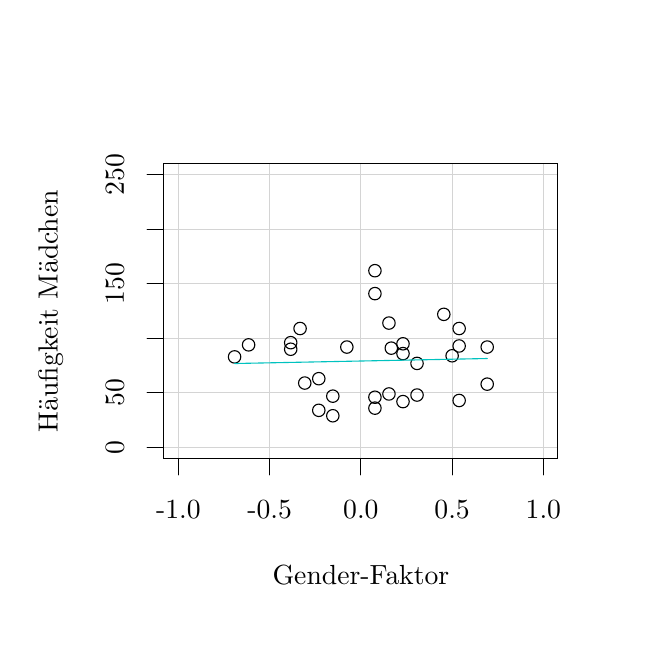
\begin{tikzpicture}[x=1pt,y=1pt]
\definecolor[named]{fillColor}{rgb}{1.00,1.00,1.00}
\path[use as bounding box,fill=fillColor,fill opacity=0.00] (0,0) rectangle (216.81,216.81);
\begin{scope}
\path[clip] (  0.00,  0.00) rectangle (216.81,216.81);
\definecolor[named]{drawColor}{rgb}{0.00,0.00,0.00}

\path[draw=drawColor,line width= 0.4pt,line join=round,line cap=round] ( 54.47, 61.20) -- (186.34, 61.20);

\path[draw=drawColor,line width= 0.4pt,line join=round,line cap=round] ( 54.47, 61.20) -- ( 54.47, 55.20);

\path[draw=drawColor,line width= 0.4pt,line join=round,line cap=round] ( 87.44, 61.20) -- ( 87.44, 55.20);

\path[draw=drawColor,line width= 0.4pt,line join=round,line cap=round] (120.41, 61.20) -- (120.41, 55.20);

\path[draw=drawColor,line width= 0.4pt,line join=round,line cap=round] (153.37, 61.20) -- (153.37, 55.20);

\path[draw=drawColor,line width= 0.4pt,line join=round,line cap=round] (186.34, 61.20) -- (186.34, 55.20);

\node[text=drawColor,anchor=base,inner sep=0pt, outer sep=0pt, scale=  1.00] at ( 54.47, 39.60) {-1.0};

\node[text=drawColor,anchor=base,inner sep=0pt, outer sep=0pt, scale=  1.00] at ( 87.44, 39.60) {-0.5};

\node[text=drawColor,anchor=base,inner sep=0pt, outer sep=0pt, scale=  1.00] at (120.41, 39.60) {0.0};

\node[text=drawColor,anchor=base,inner sep=0pt, outer sep=0pt, scale=  1.00] at (153.37, 39.60) {0.5};

\node[text=drawColor,anchor=base,inner sep=0pt, outer sep=0pt, scale=  1.00] at (186.34, 39.60) {1.0};

\path[draw=drawColor,line width= 0.4pt,line join=round,line cap=round] ( 49.20, 65.14) -- ( 49.20,163.67);

\path[draw=drawColor,line width= 0.4pt,line join=round,line cap=round] ( 49.20, 65.14) -- ( 43.20, 65.14);

\path[draw=drawColor,line width= 0.4pt,line join=round,line cap=round] ( 49.20, 84.85) -- ( 43.20, 84.85);

\path[draw=drawColor,line width= 0.4pt,line join=round,line cap=round] ( 49.20,104.55) -- ( 43.20,104.55);

\path[draw=drawColor,line width= 0.4pt,line join=round,line cap=round] ( 49.20,124.26) -- ( 43.20,124.26);

\path[draw=drawColor,line width= 0.4pt,line join=round,line cap=round] ( 49.20,143.96) -- ( 43.20,143.96);

\path[draw=drawColor,line width= 0.4pt,line join=round,line cap=round] ( 49.20,163.67) -- ( 43.20,163.67);

\node[text=drawColor,rotate= 90.00,anchor=base,inner sep=0pt, outer sep=0pt, scale=  1.00] at ( 34.80, 65.14) {0};

\node[text=drawColor,rotate= 90.00,anchor=base,inner sep=0pt, outer sep=0pt, scale=  1.00] at ( 34.80, 84.85) {50};

\node[text=drawColor,rotate= 90.00,anchor=base,inner sep=0pt, outer sep=0pt, scale=  1.00] at ( 34.80,124.26) {150};

\node[text=drawColor,rotate= 90.00,anchor=base,inner sep=0pt, outer sep=0pt, scale=  1.00] at ( 34.80,163.67) {250};

\path[draw=drawColor,line width= 0.4pt,line join=round,line cap=round] ( 49.20, 61.20) --
	(191.61, 61.20) --
	(191.61,167.61) --
	( 49.20,167.61) --
	( 49.20, 61.20);
\end{scope}
\begin{scope}
\path[clip] (  0.00,  0.00) rectangle (216.81,216.81);
\definecolor[named]{drawColor}{rgb}{0.00,0.00,0.00}

\node[text=drawColor,anchor=base,inner sep=0pt, outer sep=0pt, scale=  1.00] at (120.41, 15.60) {Gender-Faktor};

\node[text=drawColor,rotate= 90.00,anchor=base,inner sep=0pt, outer sep=0pt, scale=  1.00] at ( 10.80,114.41) {Häufigkeit Mädchen};
\end{scope}
\begin{scope}
\path[clip] ( 49.20, 61.20) rectangle (191.61,167.61);
\definecolor[named]{drawColor}{rgb}{0.83,0.83,0.83}

\path[draw=drawColor,line width= 0.4pt,line join=round,line cap=round] ( 54.47, 61.20) -- ( 54.47,167.61);

\path[draw=drawColor,line width= 0.4pt,line join=round,line cap=round] ( 87.44, 61.20) -- ( 87.44,167.61);

\path[draw=drawColor,line width= 0.4pt,line join=round,line cap=round] (120.41, 61.20) -- (120.41,167.61);

\path[draw=drawColor,line width= 0.4pt,line join=round,line cap=round] (153.37, 61.20) -- (153.37,167.61);

\path[draw=drawColor,line width= 0.4pt,line join=round,line cap=round] (186.34, 61.20) -- (186.34,167.61);

\path[draw=drawColor,line width= 0.4pt,line join=round,line cap=round] ( 49.20, 65.14) -- (191.61, 65.14);

\path[draw=drawColor,line width= 0.4pt,line join=round,line cap=round] ( 49.20, 84.85) -- (191.61, 84.85);

\path[draw=drawColor,line width= 0.4pt,line join=round,line cap=round] ( 49.20,104.55) -- (191.61,104.55);

\path[draw=drawColor,line width= 0.4pt,line join=round,line cap=round] ( 49.20,124.26) -- (191.61,124.26);

\path[draw=drawColor,line width= 0.4pt,line join=round,line cap=round] ( 49.20,143.96) -- (191.61,143.96);

\path[draw=drawColor,line width= 0.4pt,line join=round,line cap=round] ( 49.20,163.67) -- (191.61,163.67);
\end{scope}
\begin{scope}
\path[clip] (  0.00,  0.00) rectangle (216.81,216.81);
\definecolor[named]{drawColor}{rgb}{0.00,0.00,0.00}

\path[draw=drawColor,line width= 0.4pt,line join=round,line cap=round] ( 49.20, 61.20) --
	(191.61, 61.20) --
	(191.61,167.61) --
	( 49.20,167.61) --
	( 49.20, 61.20);
\end{scope}
\begin{scope}
\path[clip] ( 49.20, 61.20) rectangle (191.61,167.61);
\definecolor[named]{drawColor}{rgb}{0.00,0.00,0.00}

\path[draw=drawColor,line width= 0.4pt,line join=round,line cap=round] (166.05, 88.00) circle (  2.25);

\path[draw=drawColor,line width= 0.4pt,line join=round,line cap=round] (131.39,101.01) circle (  2.25);

\path[draw=drawColor,line width= 0.4pt,line join=round,line cap=round] (150.37,113.22) circle (  2.25);

\path[draw=drawColor,line width= 0.4pt,line join=round,line cap=round] (105.19, 78.54) circle (  2.25);

\path[draw=drawColor,line width= 0.4pt,line join=round,line cap=round] ( 98.43,108.10) circle (  2.25);

\path[draw=drawColor,line width= 0.4pt,line join=round,line cap=round] (125.48, 79.33) circle (  2.25);

\path[draw=drawColor,line width= 0.4pt,line join=round,line cap=round] (115.33,101.40) circle (  2.25);

\path[draw=drawColor,line width= 0.4pt,line join=round,line cap=round] (125.48, 83.27) circle (  2.25);

\path[draw=drawColor,line width= 0.4pt,line join=round,line cap=round] (125.48,128.99) circle (  2.25);

\path[draw=drawColor,line width= 0.4pt,line join=round,line cap=round] (135.62, 81.69) circle (  2.25);

\path[draw=drawColor,line width= 0.4pt,line join=round,line cap=round] (110.26, 76.57) circle (  2.25);

\path[draw=drawColor,line width= 0.4pt,line join=round,line cap=round] (110.26, 83.66) circle (  2.25);

\path[draw=drawColor,line width= 0.4pt,line join=round,line cap=round] ( 95.05,102.98) circle (  2.25);

\path[draw=drawColor,line width= 0.4pt,line join=round,line cap=round] (166.05,101.40) circle (  2.25);

\path[draw=drawColor,line width= 0.4pt,line join=round,line cap=round] ( 79.83,102.19) circle (  2.25);

\path[draw=drawColor,line width= 0.4pt,line join=round,line cap=round] ( 95.05,100.61) circle (  2.25);

\path[draw=drawColor,line width= 0.4pt,line join=round,line cap=round] (125.48,120.71) circle (  2.25);

\path[draw=drawColor,line width= 0.4pt,line join=round,line cap=round] (155.91, 82.09) circle (  2.25);

\path[draw=drawColor,line width= 0.4pt,line join=round,line cap=round] (105.19, 89.97) circle (  2.25);

\path[draw=drawColor,line width= 0.4pt,line join=round,line cap=round] ( 74.76, 97.85) circle (  2.25);

\path[draw=drawColor,line width= 0.4pt,line join=round,line cap=round] (100.12, 88.39) circle (  2.25);

\path[draw=drawColor,line width= 0.4pt,line join=round,line cap=round] (130.55,110.07) circle (  2.25);

\path[draw=drawColor,line width= 0.4pt,line join=round,line cap=round] (130.55, 84.45) circle (  2.25);

\path[draw=drawColor,line width= 0.4pt,line join=round,line cap=round] (140.69, 84.06) circle (  2.25);

\path[draw=drawColor,line width= 0.4pt,line join=round,line cap=round] (135.62,102.58) circle (  2.25);

\path[draw=drawColor,line width= 0.4pt,line join=round,line cap=round] (155.91,101.79) circle (  2.25);

\path[draw=drawColor,line width= 0.4pt,line join=round,line cap=round] (135.62, 99.03) circle (  2.25);

\path[draw=drawColor,line width= 0.4pt,line join=round,line cap=round] (140.69, 95.49) circle (  2.25);

\path[draw=drawColor,line width= 0.4pt,line join=round,line cap=round] (155.91,108.10) circle (  2.25);

\path[draw=drawColor,line width= 0.4pt,line join=round,line cap=round] (153.37, 98.25) circle (  2.25);
\definecolor[named]{drawColor}{rgb}{0.00,0.76,0.75}

\path[draw=drawColor,line width= 0.4pt,line join=round,line cap=round] ( 74.76, 95.45) --
	(166.05, 97.26);
\end{scope}
\end{tikzpicture}
